%%
%  ******************************************************************************
%  * #file    Szablon_raportu_EN_Latex.tex
%  * #author  Adrian Wójcik   adrian.wojcik(at)put.poznan.pl
%  *          
%  * #commit  Patryk Kościk   koscikpatryk(at)gmail.com
%  *          Modified the template for Projekt przejsciowy purposes          
%  *          
%  * #version 1.0
%  * #date    09-Mar-2022
%  * #brief   PROJPRZEJ
%  *
%  ******************************************************************************
%%  
\documentclass[11pt, a4paper]{article}

\usepackage{setup}

% Wypełnijcie te dyrektywy zgodnie z waszym tematem
% \lab      -> NAZWA CZUJNIKA, np.: 'DHT22'
% \comment  -> Króciutki opis co to, np.: 'Cyfrowy budżetowy czujnik temperatury'
%
\lab{Czujnik dymu}
\comment{Moduł czujnika dymu i łatwopalnych gazów MQ-2}
\author{Adam Rewekant}

% Absolutny zakaz dotykania tego tutaj bo jak dotkiecie to coś jebnie
\university{Politechnika Poznańska}
\faculty{Wydział Automatyki, Robotyki i Elektrotechniki}
\institute{Instytut Robotyki i Inteligencji Maszynowej}
\department{Zakład Sterowania i Elektroniki Przemysłowej}
\addbibresource{bib/elem.bib}
\nocite{*}

%%
%
% Początek dokumentu
%
%%
\begin{document}

%% Strona tytułowa %%
\mainpage{{fig/element/mainfot}}

\newpage
\section*{Opis elementu} \addcontentsline{toc}{section}{Wstęp}
Moduł czujnika dymu MQ-2 to czujnik wykrywający zmianie rezystancji materiału czujnika w momencie kontaktu gazu z materiałem. Stężenie gazu można wykryć za pomocą prostej sieci dzielników napięcia. 



\vspace{0.5cm}
\begin{figure}[h]
\centering
\begin{subfigure}{.5\textwidth}
  \centering
  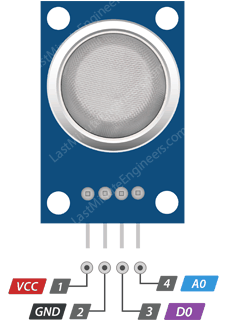
\includegraphics[width=.6\linewidth]{fig/element/pinfot.png}
  \caption{Moduł czujnika MQ-2 \cite{fot1}}
  \label{fig:sub1}
\end{subfigure}%
\begin{subfigure}{.5\textwidth}
  \centering
  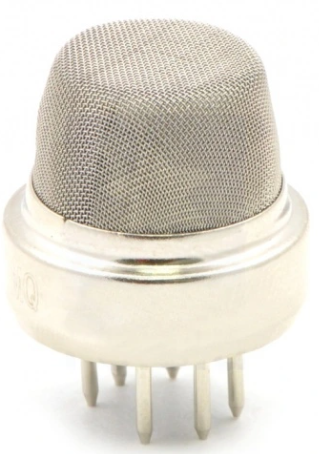
\includegraphics[width=.6\linewidth]{fig/element/elemfot.png}
  \caption{Moduł czujnika MQ-2 \cite{fot2}}
  \label{fig:sub2}
\end{subfigure}
\caption{Przykładowe zdjęcia czujnika.}
\label{fig:test}
\end{figure}
\vspace{0.5cm}

Konstrukcja czujnika oparta jest na dwutlenku krzemu (SnO2). W momencie wykrycia gazu lub dymu natychmiastowo spada rezystancja. Na płytce znajduje się prosty układ komparatora, który zapewnia dodatkowe wyjście cyfrowe z regulowanym progiem przełączania. Służy do tego potencjometr, który również znajduje się na płytce.

Czujnik posiada także wyjście analogowe, które należy podłączyć do wyprowadzenia przetwornika A/C. Pozwoli to mierząc proporcjonalny sygnał napięciowy, dokładniej określić stężenie.


\begin{figure}[h]
\centering
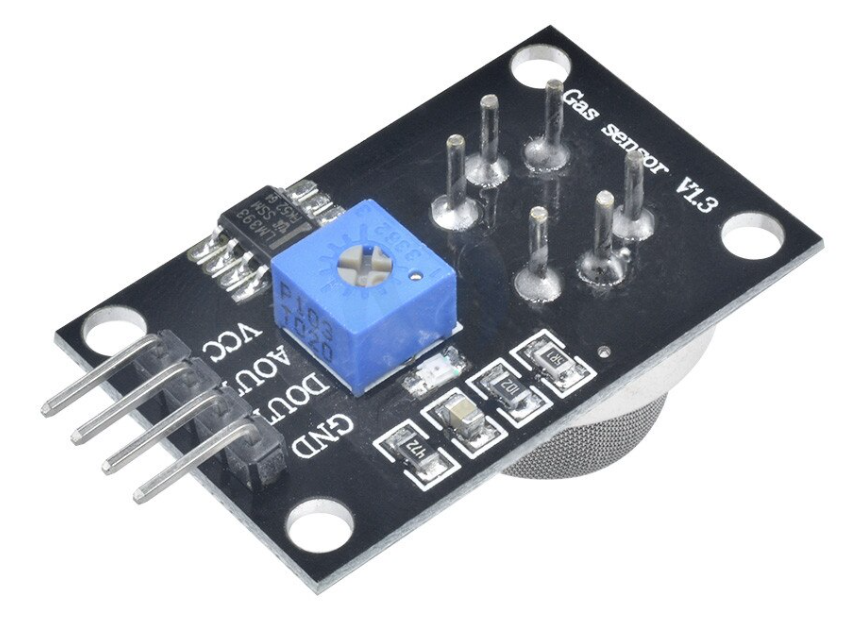
\includegraphics[width=.6\linewidth]{fig/element/backfot.png}
\caption{Zdjęcie tyłu czujnika.\cite{fot3}}
\label{fig:test}
\end{figure}
\vspace{0.5cm}



\newpage
\begin{figure}[h]
\centering
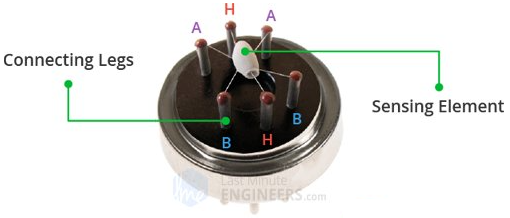
\includegraphics[width=.7\linewidth]{fig/element/infot.png}
\caption{Budowa czujnika.\cite{fot2}}
\label{fig:test}
\end{figure}
\vspace{0.5cm}
Tak wygląda czujnik po zdjęciu zewnętrznej siatki. Struktura w kształcie gwiazdy jest utworzona przez element czujnikowy i sześć nóżek łączących, które wystają poza bakelitową podstawę. Spośród tych sześciu przewodów dwa (H) odpowiadają za ogrzewanie elementu czujnikowego i są połączone za pomocą cewki niklowo-chromowej, dobrze znanego stopu przewodzącego.\\

Pozostałe cztery przewody (A i B) odpowiedzialne za sygnały wyjściowe są połączone za pomocą przewodów platynowych. Przewody te są podłączone do korpusu elementu czujnikowego i przenoszą niewielkie zmiany w prądzie przepływającym przez element czujnikowy.
\vspace{2cm}
\begin{figure}[h]
\centering
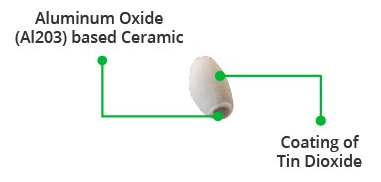
\includegraphics[width=.5\linewidth]{fig/element/ininfot.png}
\caption{Budowa czujnika.\cite{fot2}}
\label{fig:test}
\end{figure}
\vspace{0.5cm}

Rurkowy element pomiarowy jest wykonany z ceramiki na bazie tlenku glinu (AL2O3) i pokryty powłoką z dwutlenku cyny (SnO2). Dwutlenek cyny jest najważniejszym materiałem, ponieważ jest wrażliwy na gazy palne. Jednak podłoże ceramiczne zwiększa wydajność ogrzewania i zapewnia stałe nagrzewanie obszaru czujnika do temperatury roboczej.
\newpage
\begin{figure}[h!]
    \centering
    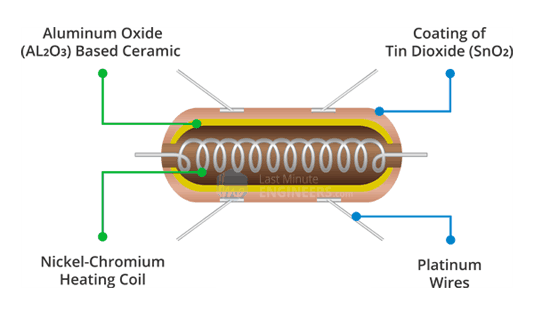
\includegraphics[width=0.8\linewidth]{fig/element/structfot.png}
    \caption{Budowa czujnika.\cite{fot2}}
    \label{fig:my_label}
\end{figure}
\vspace{0.5cm}
Cewka niklowo-chromowa i ceramika na bazie tlenku glinu tworzą układ grzewczy, a druty platynowe i powłoka z dwutlenku cyny tworzą układ detekcji.
\section{Użycie czujnika}

\vspace{0.5cm}
\begin{figure}[h!]
    \centering
    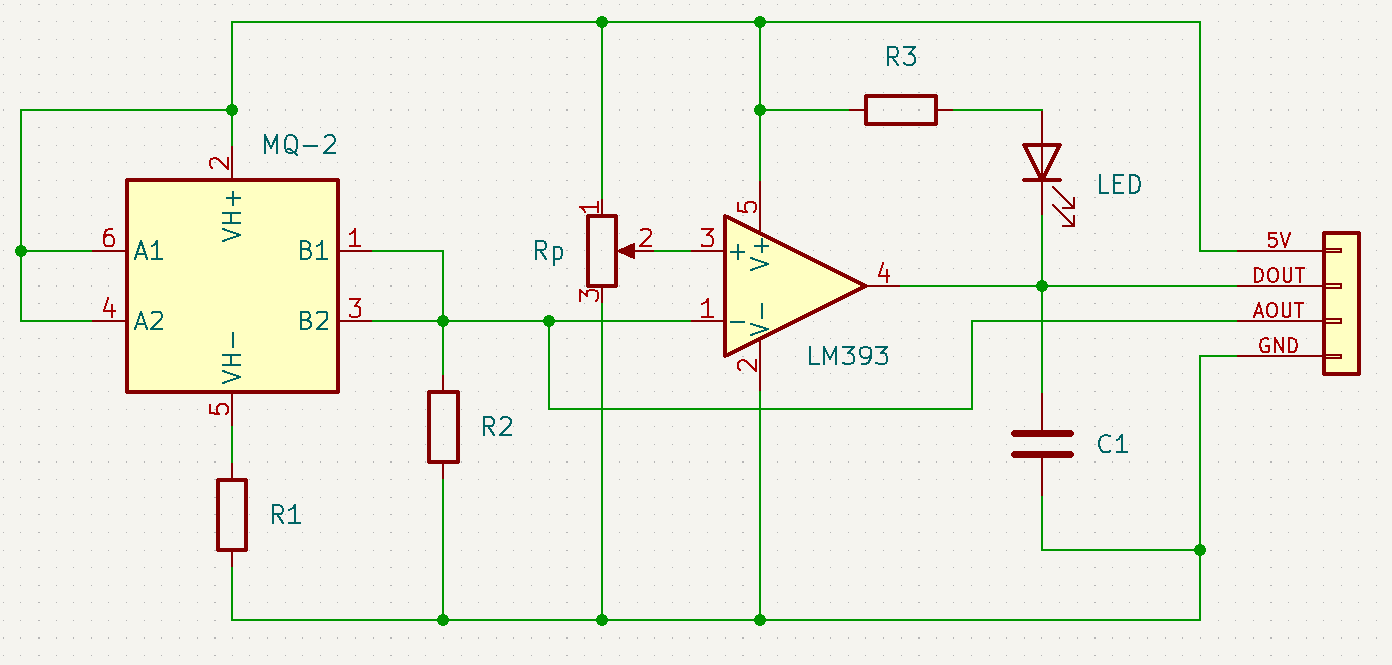
\includegraphics[width=\linewidth]{fig/element/kicadfot.png}
    \caption{Połaczenie elektryczne}
    \label{fig:my_label}
\end{figure}
\vspace{0.5cm}

Czujnik dymu, wykorzystywany jest najczęściej w systemach alarmowych, ochronie przeciwpożarowej.

\newpage
\section{Prezentacja działania układu}

\vspace{0.5cm}
\begin{figure}[h!]
    \centering
    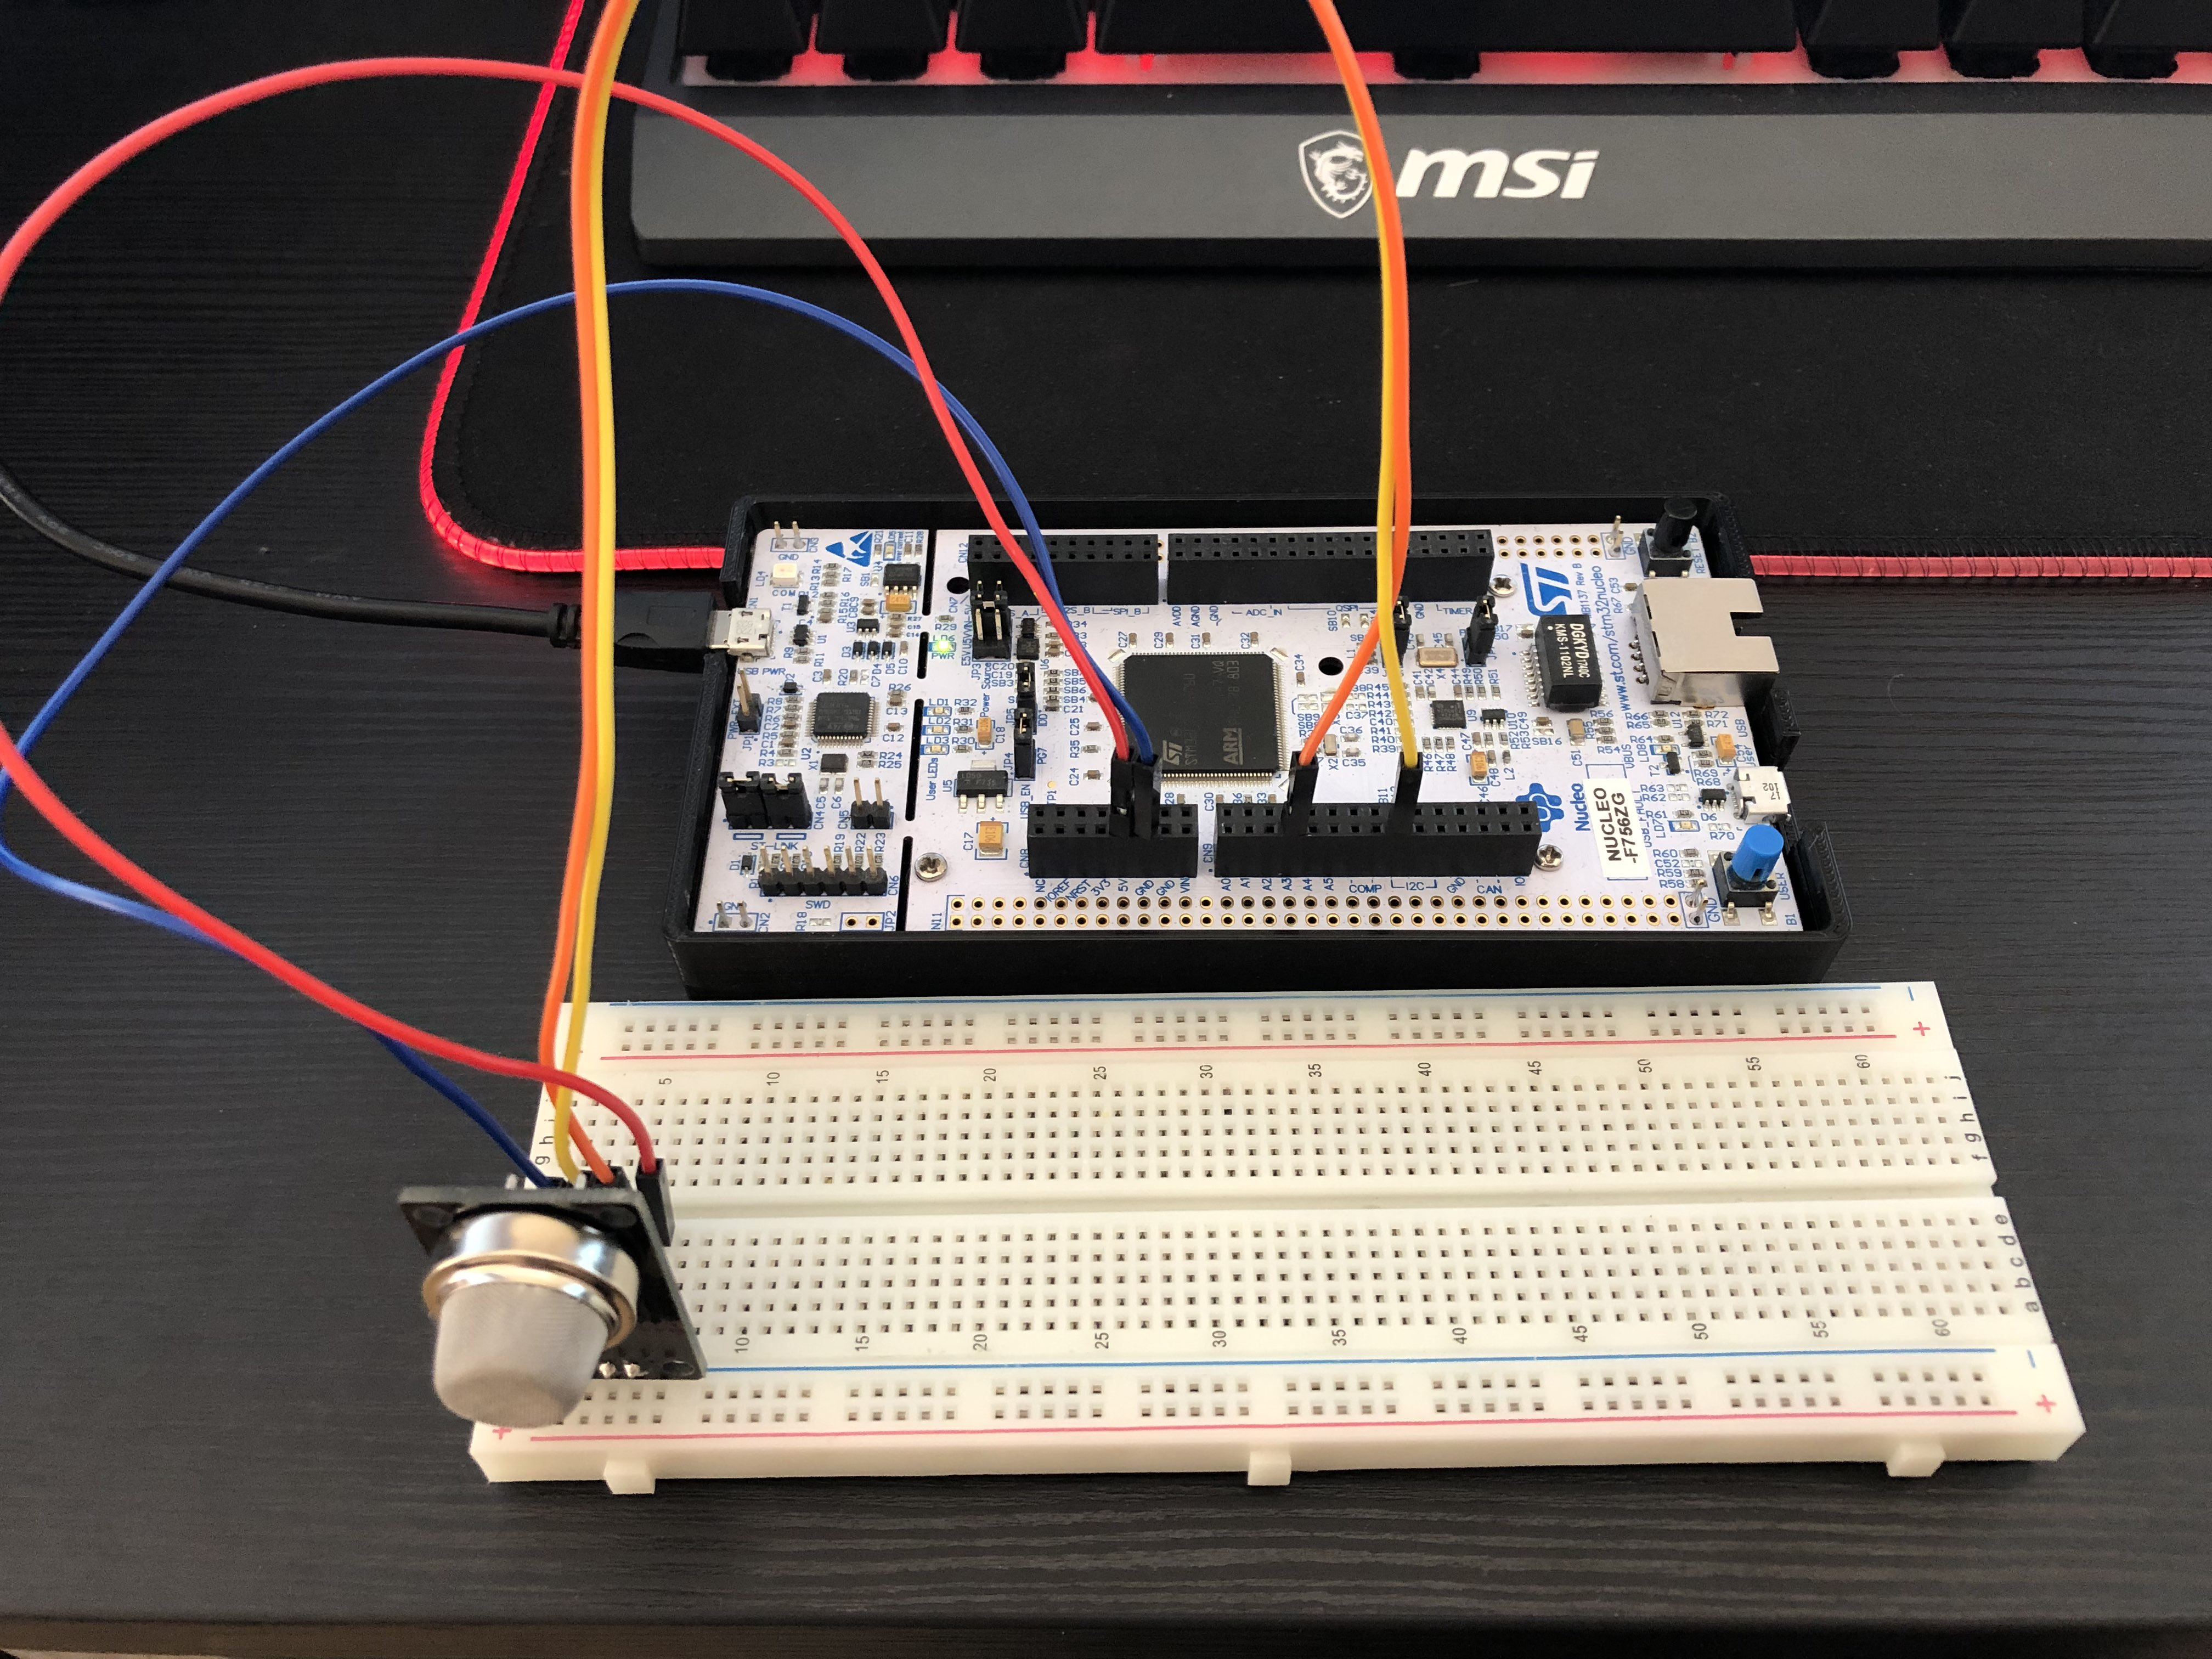
\includegraphics[width=\textwidth]{fig/element/off.png}
    \caption{Zdjęcie układu - brak wykrycia dymu lub łatwopalnego gazu.}
    \label{fig:my_label}
\end{figure}
\vspace{0.5cm}
\begin{figure}[h!]
    \centering
    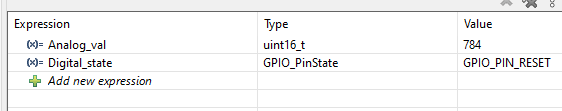
\includegraphics[width=\textwidth]{fig/element/sensoff.png}
    \caption{Zdjęcie pomiaru - brak wykrycia dymu lub łatwopalnego gazu.}
    \label{fig:my_label}
\end{figure}

\vspace{0.5cm}
\begin{figure}[h!]
    \centering
    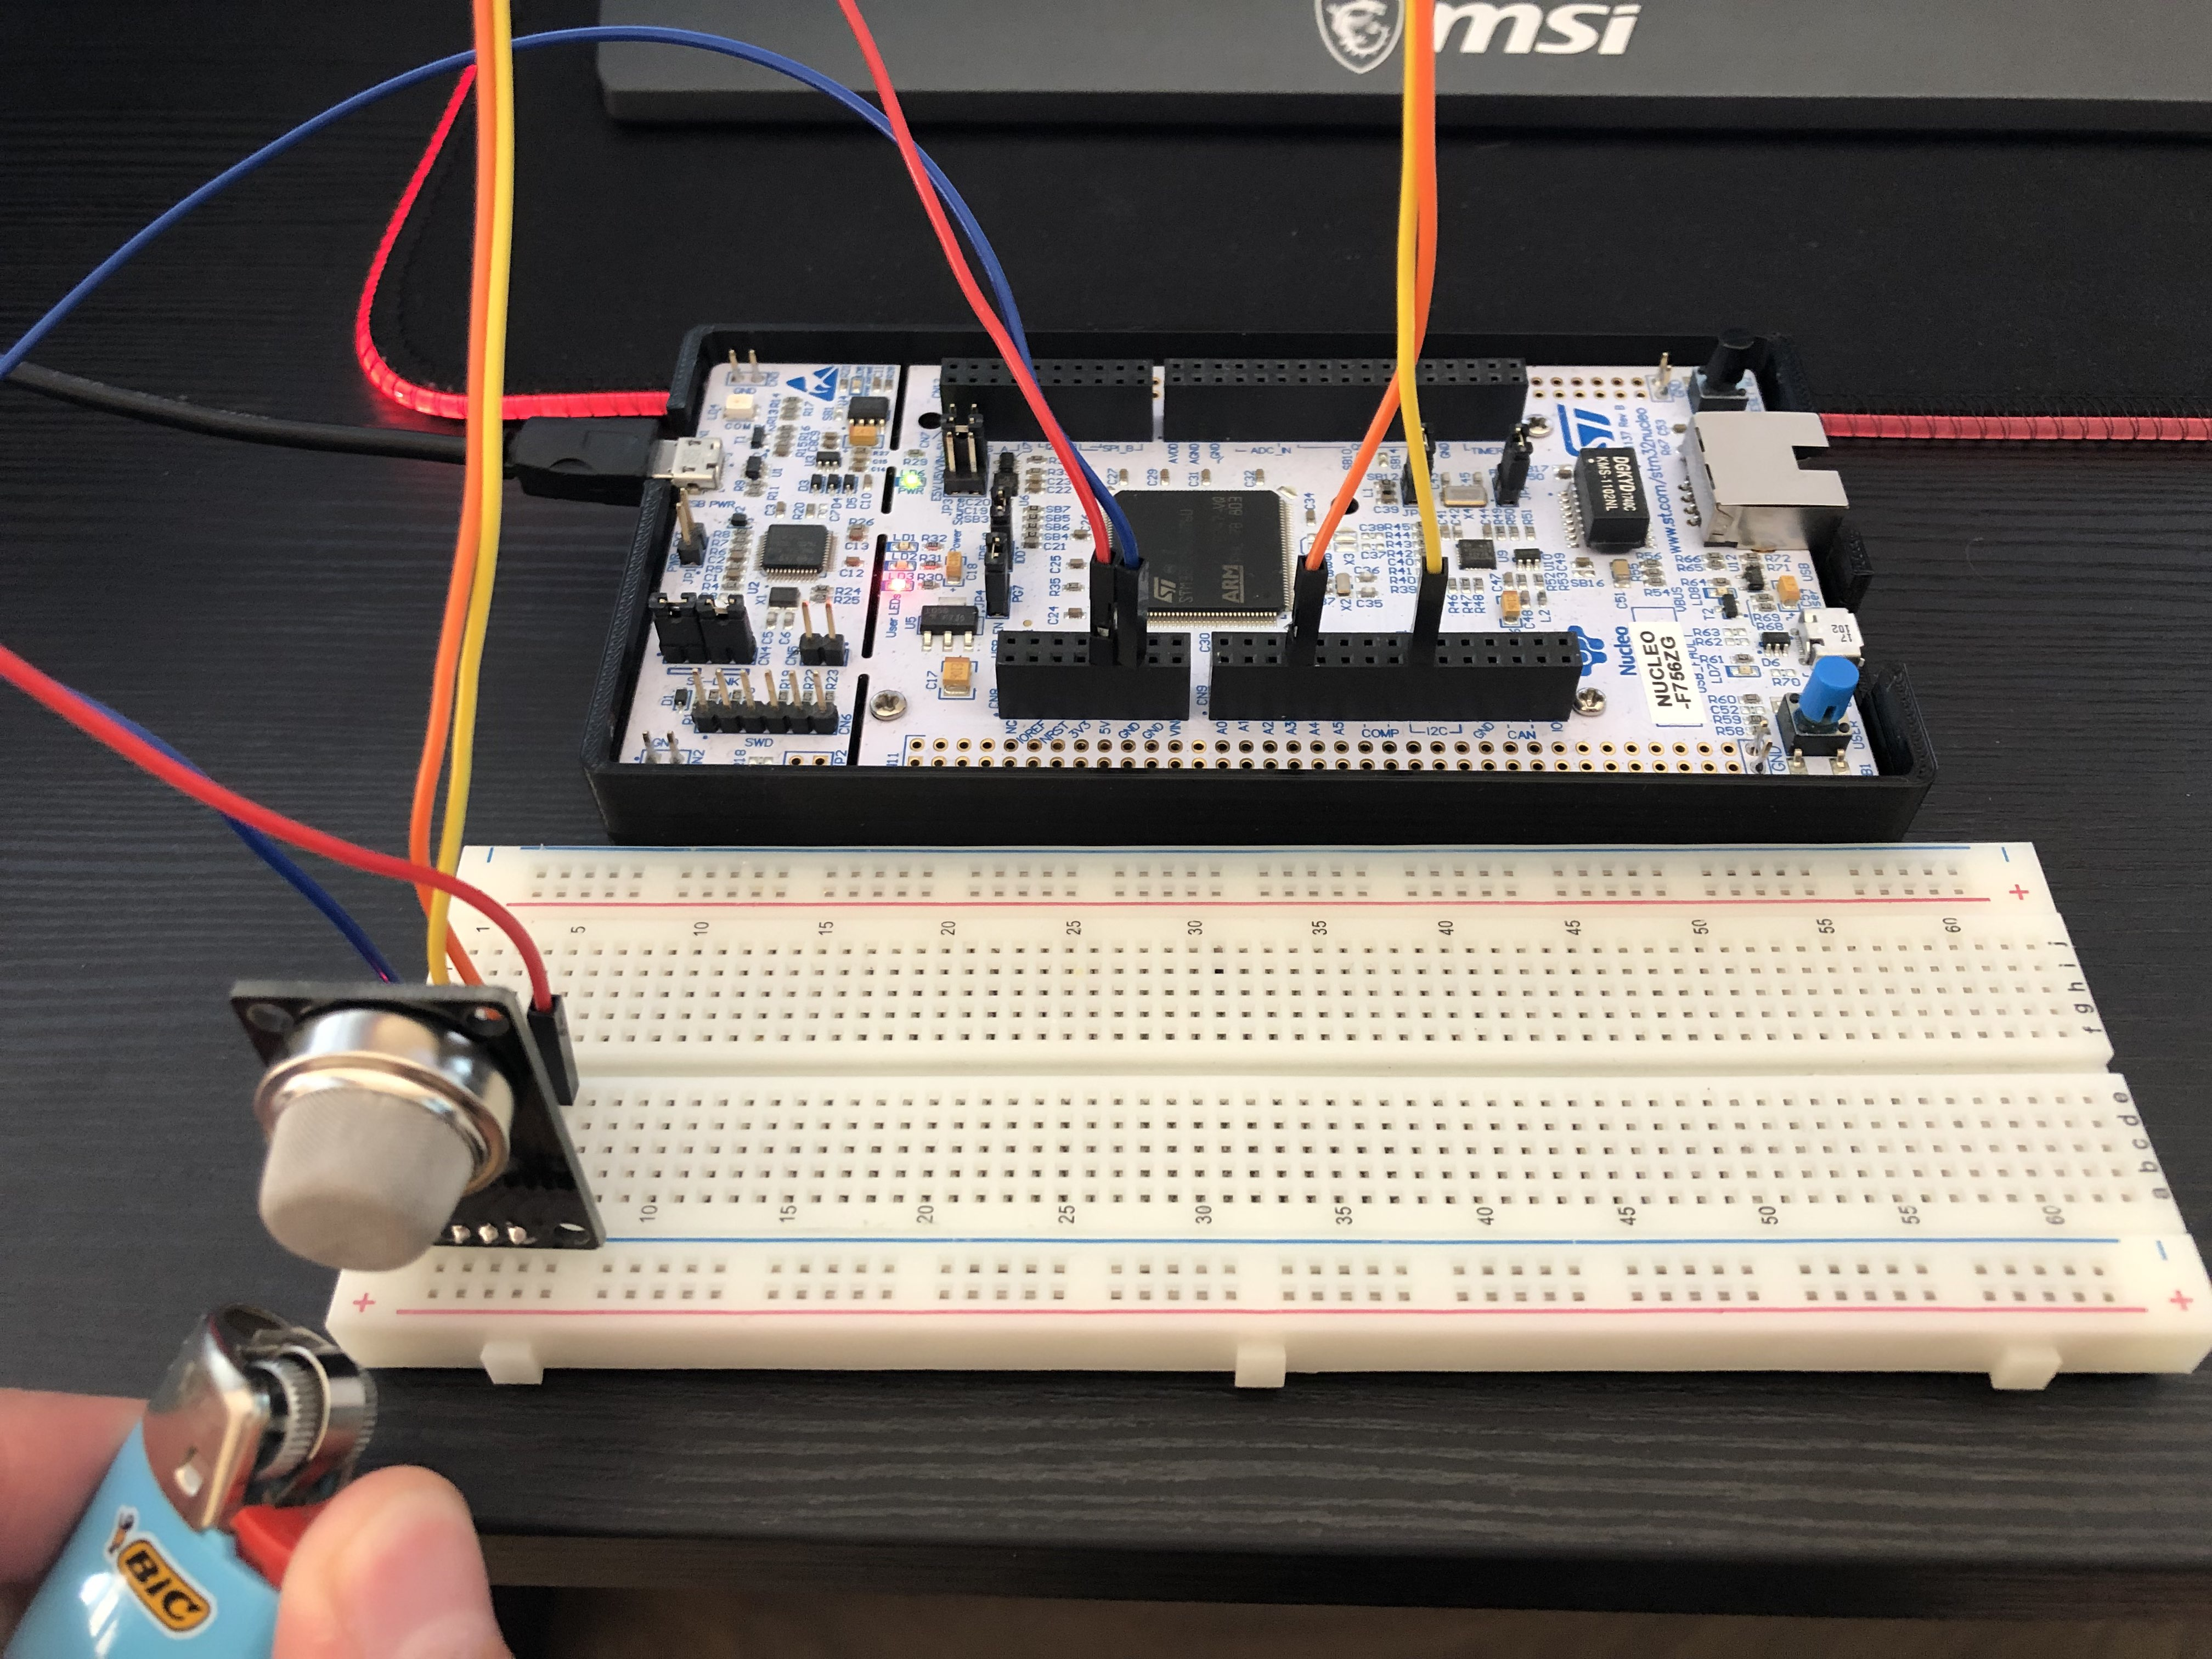
\includegraphics[width=\textwidth]{fig/element/on.png}
    \caption{Zdjęcie układu - wykrycie dymu lub łatwopalnego gazu.}
    \label{fig:my_label}
\end{figure}
\vspace{0.5cm}
\begin{figure}[h!]
    \centering
    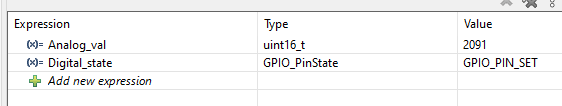
\includegraphics[width=\textwidth]{fig/element/senson.png}
    \caption{Zdjęcie pomiaru - wykrycie dymu lub łatwopalnego gazu.}
    \label{fig:my_label}
\end{figure}
\newpage
Działanie czujnika zostało zaprezentowane na krótkim wideo. \cite{youtube}.
\newpage
\printbibliography[heading=bibintoc]

\end{document}
